\chapter{Firewall}
Die Firewall wird in dem Praktikum mit IPTables von Linux realisiert. Dies ermöglicht das Aufstellen von Regeln, welche in Tabellen abgelegt werden, um Verbindungen zwischen zwei Netzen zu kontrollieren. Wenn ein Paket die Firewall erreicht, dann checkt die Firewall sequentiell die einzelnen Regeln und wenn eine Zutrifft wird der zugehörige ACCEPT oder DROP auf das Paket angewandt. Bei ACCEPT wird das Paket weiter gereicht und bei DROP wird das Paket einfach fallen gelassen und der Zielrechner erhält nicht das Paket. Wenn keine Regel zutrifft, dann wird die Default Policy angewandt. Diese kann wiederum auf DROP und ACCEPT gesetzt sein. 
\begin{figure}
	\centering
		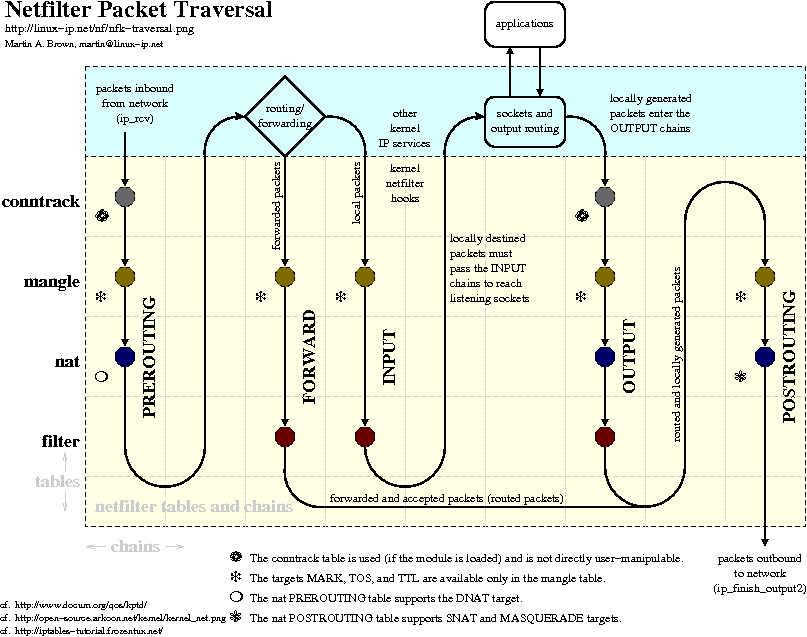
\includegraphics[width=1.00\textwidth]{figures/firewall_uebersicht.PNG}
	\caption{Firewall Übersicht \cite{linux-ip}}
	\label{fig:firewall_uebersicht}
\end{figure}
In der Abbildung \ref{fig:firewall_uebersicht} ist zu sehen das es verschiedene Tabellen gibt. Je nachdem ob des Paket weitergeleitet wird oder einen lokalen Prozess als Ziel hat, werden die zuständigen Tabellen geprüft. Folgend eine kurze Erklärung, wann welche Tabelle genutzt wird.
\begin{itemize}
	\item PREROUTING \\
	Hier landen Pakete bevor entschieden worden ist, ob das Paket weitergeleitet wird oder einen lokalen Prozess als Ziel hat.
	\item POSTROUTING \\
	Ganz zum schluss, wenn schon alle vorherigen Entscheidungen getroffen worden sind wird laufen die Pakete hier nochmals durch.
	\item FORWARD \\
	Hierbei handelt es sich um ein Paket, welches weitergeleitet wird.
	\item INPUT \\
	Das Paket hat einen lokalen Prozess, auf dem Rechner wo die Firewall läuft, als Ziel.
	\item OUTPUT \\
	Hierbei handelt es sich um ein Paket, welche von einem lokalen Prozess abgesendet wird.
\end{itemize}
Die Regeln beschränken sich auf die Schicht 3 und 4 von den zu übertragenden Paketen. Somit hat man Zugriff auf die Übertragungsflags, IP-Adressen, Ports und die zugehörigen Netzwerkinterfaces. IPTables ermöglicht verbindungsorientierte Paketfilter, somit kann zum Beispiel überprüft werden ob eine Verbindung related ist, dass heißt es wird eine Unterverbindung aufgebaut, wo schon eine Verbindung zwischen den Rechnern besteht. Des weiteren ermöglicht IPTables eine NAT mit Masquerade Funktion. Das bedeutet es versteckt die Rechner von einem Netzwerk vor dem anderen.

\section{Anforderungen}
Indem Praktikumsaufbau gibt es zwei Firewalls. Hierbei handelt es sich um eine Äußere Firewall, welche wie in Abbildung \ref{fig:Netzplan} zu erkennen die Verbindungen zwischen der DMZ und dem Internet regelt. Und die Rechner aus der DMZ werden vor Rechnern aus dem Internet versteckt. Die innere Firewall hat dabei dieselben Aufgaben nur ist sie zwischen der DMZ und dem Firmennetzwerk platziert.

\subsection{Äußere Firewall (FW1)}
\begin{itemize}
\item Masquerading von der DMZ zum Internet.
\item Der Webserver aus der DMZ soll von dem Internet über die üblichen Ports erreichbar sein. Darunter fallen folgende Ports. 80(HTTP), 443(HTTPS), 25(SMTP), 587(SMTP), 465(SMTPS), 993(IMAPS), 995(POP3S), 143(IMAP), 110(POP3), 53(DNS)
\item Die interne Firewall muss erreichbar sein für das VPN. Somit müssen folgende Ports auf die innere Firewall weitergeleitet werden. 1195(VPN: Client to Lan), 1194(VPN: Lan to Lan)
\end{itemize}

\subsection{Innere Firewall (FW2)}
\begin{itemize}
\item Masquerading von dem Firmennetz zur DMZ. Somit dürfen die IP Adressen der Rechner aus dem Firmennetz in der DMZ nicht erkennbar sein, sondern als IP Adresse ist die der Firewall zu sehen.
\item Es dürfen keine neuen Verbindungen von der DMZ in das interne Firmennetz aufgebaut werden.
\item Rechner aus dem Firmen internen Netzwerk dürfen neue Verbindungen zur DMZ und dem Internet aufbauen.
\item Auf der inneren Firewall läuft der VPN Prozess und dieser muss aus dem Internet erreichbar sein.	
\end{itemize}

\section{Implementierung}
Damit die Praktikumsaufgabe reibungslos bearbeitet werden kann, wurde zu Anfang das NAT/Masquerading eingerichtet. Daraufhin wurde das VPN eingerichtet und getestet. Und sobald alle Funktionalitäten geprüft waren, wurde der Paketfilter eingerichtet. Durch diese Reihenfolge konnte sichergestellt werden, dass der Paketfilter von der Firewall nicht die Funktionalität des VPN Dienstes stört.

IPTables speichert seine Tabelleneinträge nur im Arbeitsspeicher, deswegen sind die Einträge welche hinzugefügt werden nach einem Neustart des Rechners wieder verschwunden. Damit die Einträge gespeichert werden, müssen diese mittels dem iptables-save Befehl in eine Datei gespeichert werden. 
\begin{lstlisting}
iptables-save > /etc/iptables.rules
\end{lstlisting}
Durch diesen Befehl werden alle IPTables Einträge in /etc/iptables.rules gespeichert. Damit nach einem Neustart diese Einträge auch geladen werden, muss unter /etc/network/if-pre-up.d/ ein ein Skript erstellt werden, welches die gespeicherten Einträge mittels iptables-restore aus der Datei lädt. Debian führt alles ausführbaren Skripte in dem Ordner if-pre-up.d aus bevor die Netzwerkdienste gestartet werden. Das Skript sieht wie folgt aus:
\begin{lstlisting}[caption={/etc/network/if-pre-up.d/iptables}]
iptables-restore < /etc/iptables.rules
\end{lstlisting}
Mit dem Befehl "chmod +x" wurde bei dem Skript das ausführbar Flag gesetzt. Somit werden die IPTables Regeln aus der Datei /etc/iptables.rules bei jedem Start des Rechners geladen. Somit können die IPTables mit normalen Befehlen eingerichtet werden und durch den iptables-save Befehl werden. Dieses Konfiguration wurde auf beiden Rechnern eingerichtet.

\subsection{ICMP}
Das Internet Control Message Protkoll dient dazu um Informationen und Fehlermeldungen über das Netzwerk zu übertragen. Wenn zum Beispiel ein Paket verworfen wird, dann kann dies mittels einer ICMP Nachricht demjenigen der versucht eine Verbindung aufzubauen mitgeteilt werden. Diese Informationen sind zum warten und testen eines Systems sehr praktisch. Jedoch auch für einen Angreifer können diese Informationen sinnvoll sein. Auf diesen Rechnern wurden diese Pakete erlaubt, damit mittels "Ping" getestet werden kann, welche Rechner erreichbar sind. Somit wurden folgende Input Pakete erlaubt.
\lstinputlisting[
    firstline=9,
    lastline=9,
    label = fw:fw1_iptables_icmp,
    caption={FW1 iptables.rules - Ausschnitt ICMP Paketfilter}
]{code/fw1_iptables.rules}
Dasselbe wurde auf der zweiten Firewall auch eingerichtet. Somit sind die Firewall Rechner weiterhin zu pingbar. Man kann diesen Filter auch entfernen, wenn man sich sicher ist, dass alles in Ordnung läuft. Jedoch bei auftretenden Fehlern erschwert es einem die Fehlersuche. Für dieses Praktikum war die erleichterte Fehlersuche der Hauptgrund für das erlauben dieser Pakete.

\subsection{NAT / Masquerading}
Das Einrichten von Masquerading erfolgte auf beiden Firewall Rechnern gleich, da diese Funktionalität auf beiden die selbe ist. Die Netzwerkschnittstelle "eth0" ist mit dem Netzwerk verbunden, welches versteckt werden soll. Wobei "eth1" mit dem Netzwerk verbunden ist, welchem nicht zu vertrauen ist. Das ist einmal die DMZ von dem firmeninternen Netzwerk und das Internet gesehen von der DMZ. \\
Als erstes musste unter /etc/sysctl.config das Forwarding der Pakete aktiviert werden. Dies erfolgte mit dem ändern des ipv4 forward Flags.
\begin{lstlisting}[caption={/etc/sysctl.config}]
net.ipv4.ip_forward=1
\end{lstlisting}
Somit ist das weiterleiten der Pakete ermöglicht. Das Masquerading wird dann mittels iptables realisiert. Dafür muss folgender Eintrag hinzugefügt werden.
\begin{lstlisting}
iptables -t nat -A POSTROUTING -o eth1 -j MASQUERADE
\end{lstlisting}
Durch diesen Eintrag wird eth1 als Output Interface für das Masquerading verwendet. Dieser Eintrag wird in die spezielle NAT Tabelle eingetragen.

\subsection{Implementierung FW1}
Diese Firewall regelt die Verbindung zwischen der DMZ und dem Internet. Somit ist es wichtig das Pakete welche an bestimmten Ports ankommen auch an den zutreffenden Server weitergeleitet werden. In diesem Praktikum ist das der srv1.firma-a.f223 mit der IP-Adresse "192.168.40.1". Das bedeutet es müssen zuerst die Pakete welche an die Firewall ankommen in der PREROUTING Kette weitergeleitet werden. In der Auflistung \ref{fw:fw1_iptables_prerouting} sind Einträge für die Nat Tabelle in der Kette Prerouting zu erkennen. Es wird anhand des ankommenden Netzwerkinterfaces und Port entschieden ob das Paket weitergeleitet wird an den Webserver. Hier wurden alle relevanten Ports eingetragen.
\lstinputlisting[
    firstline=35,
    lastline=47,
    label = fw:fw1_iptables_prerouting,
    caption={FW1 iptables.rules - NAT Prerouting}
]{code/fw1_iptables.rules}
Ebenso werden die udp Pakete welche für das VPN zuständig sind, an die innere Firewall weitergeleitet mit der IP-Adresse "192.168.40.250". Diese Pakete welche weitergeleitet werden, kommen somit an die Paketfilter Regeln an der Kette FORWARD. Damit diese dort nicht einfach verworfen werden, müssen die Ports in dieser Kette ebenfalls eingetragen werden. Dies ist in folgenden Auflistung zu sehen.
\lstinputlisting[
    firstline=10,
    lastline=24,
    label = fw:fw1_iptables_forward,
    caption={FW1 iptables.rules - Paketfilter Forward}
]{code/fw1_iptables.rules}
Somit werden Pakete alle Pakete akzeptiert, welche den state "NEW" haben und aus dem Internet auf den Webserver weitergeleitet werden. Das sind die Zeilen 3 bis 13 in der Auflistung \ref{fw:fw1_iptables_forward}. Die Zeilen 14 und 15 sind wiederum für die Pakete vom VPN Dienstes zuständig. Die erste Zeile erlaubt, dass Pakete von der DMZ zum Internet erlaubt sind. Die zweite Zeile erlaubt 